% This file was created with tikzplotlib v0.10.1.
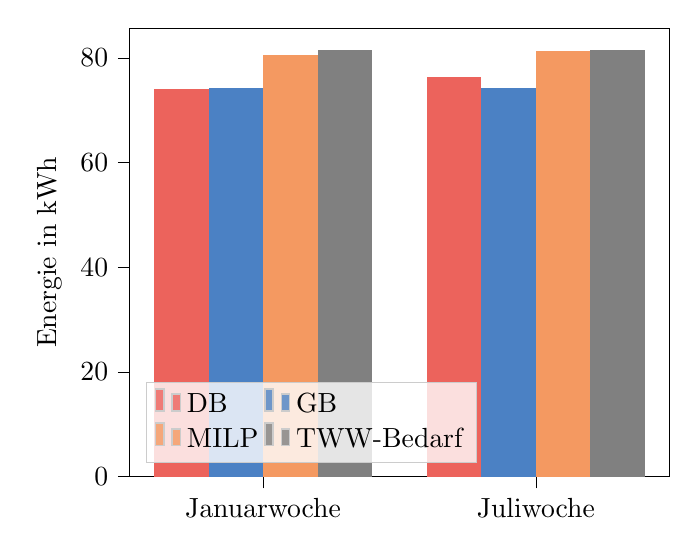
\begin{tikzpicture}

\definecolor{darkgray176}{RGB}{176,176,176}
\definecolor{gray}{RGB}{128,128,128}
\definecolor{lightgray204}{RGB}{204,204,204}
\definecolor{sandybrown24415397}{RGB}{244,153,97}
\definecolor{steelblue75129196}{RGB}{75,129,196}
\definecolor{tomato2369992}{RGB}{236,99,92}

\begin{axis}[
legend cell align={left},
legend columns=2,
legend style={
  fill opacity=0.8,
  draw opacity=1,
  text opacity=1,
  at={(0.03,0.03)},
  anchor=south west,
  draw=lightgray204
},
tick align=outside,
tick pos=left,
x grid style={darkgray176},
xmin=0.51, xmax=2.49,
xtick style={color=black},
xtick={0.999,1.9999999999999},
xticklabels={Januarwoche,Juliwoche},
y grid style={darkgray176},
ylabel={Energie in kWh},
ymin=0, ymax=85.66425,
ytick style={color=black}
]
\draw[draw=none,fill=tomato2369992,semithick] (axis cs:0.6,0) rectangle (axis cs:0.8,74.135);
\addlegendimage{ybar,ybar legend,draw=none,fill=tomato2369992,semithick}
\addlegendentry{DB}

\draw[draw=none,fill=tomato2369992,semithick] (axis cs:1.6,0) rectangle (axis cs:1.8,76.335);
\draw[draw=none,fill=steelblue75129196,semithick] (axis cs:0.8,0) rectangle (axis cs:1,74.235);
\addlegendimage{ybar,ybar legend,draw=none,fill=steelblue75129196,semithick}
\addlegendentry{GB}

\draw[draw=none,fill=steelblue75129196,semithick] (axis cs:1.8,0) rectangle (axis cs:2,74.235);
\draw[draw=none,fill=sandybrown24415397,semithick] (axis cs:1,0) rectangle (axis cs:1.2,80.535);
\addlegendimage{ybar,ybar legend,draw=none,fill=sandybrown24415397,semithick}
\addlegendentry{MILP}

\draw[draw=none,fill=sandybrown24415397,semithick] (axis cs:2,0) rectangle (axis cs:2.2,81.27);
\draw[draw=none,fill=gray,semithick] (axis cs:1.2,0) rectangle (axis cs:1.4,81.585);
\addlegendimage{ybar,ybar legend,draw=none,fill=gray,semithick}
\addlegendentry{TWW-Bedarf}

\draw[draw=none,fill=gray,semithick] (axis cs:2.2,0) rectangle (axis cs:2.4,81.585);
\end{axis}

\end{tikzpicture}
